% Introduction
\section{Introduction}

%%%%%%

% Cite:
% Wireless networks			#gupta2000capacity
% Wireless sensor networks	#akyildiz2002wireless
% Volcanic investigation		#werner2006deploying

% Mobile campus networks 	#hernandez2005comparative
% Mobile gaming community	#cunningham2002optimizing
% Energy-efficient network	#jones2001survey
% Internet of things 			#qin2014software
% Connectivity  			#moscibroda2006complexity
% Density					#wang2015connectivity
% Unit disk graph model 		#clark1990unit
% CSMA/CA				#bianchi1996performance

% The cite of the existing algorithms are listed in related work

%%%%%%

% Paper Logic Flow

% Background and topic: Neighbor discovery in an energy-restricted large-scale network
% Wireless sensor networks and practical scenario 
The popularity of Internet of Things (IoT) has turned people's attention back to wireless sensor networks\cite{akyildiz2002wireless}, with a wide range of applications such as volcanic investigation \cite{werner2006deploying}, seismic detection \cite{suzuki2007high}, agriculture monitoring \cite{wang2010l3sn}, etc. 

Neighbor discovery, in which a node tends to discover its nearby neighboring nodes before further applications like broadcasting and peer-to-peer communication, is a fundamental step to construct a wireless sensor network. In this paper, we study it in an energy-restricted large-scale scenario, where nodes are aware of energy consumption and multi-hop connected.


%The existing algorithms and their weakness in an energy-restricted large-scale network
Unfortunately, despite great efforts, neighbor discovery in a large-scale network is still an open problem.
The existing algorithms can be classified into two categories: deterministic, and probabilistic.
In the deterministic algorithms \cite{dutta2008practical, kandhalu2010u, bakht2012searchlight, sun2014hello,  chen2015heterogeneous}, sensors take actions based on deterministic sequences.
Nevertheless, most deterministic algorithms are designed only for two nodes and directly applied to multi-node scenario. Probabilistic algorithms handle neighbor discovery in a clique of $n$ nodes\cite{mcglynn2001birthday, vasudevan2009neighbor, you2011aloha, song2014probabilistic} , i.e. every two nodes are neighbors, and utilize the global number $n$ to compute an optimal probability for action decisions. However in a large-scale network, a node is only able to sense nodes within a distance range. In addition, some existing algorithms \cite{mcglynn2001birthday,vasudevan2009neighbor} do not consider energy consumption of the neighbor discovery process. In wireless sensor networks, sensors have limited energy and are recharged frequently. Attempting for neighbor discovery process consistently will be energy-consuming. 

%The main challenges in an energy-restricted large-scale network
Therefore, we look into the existing neighbor discovery algorithms and find that the key issue lies in collisions in the large-scale networks (collisions result in CSMA \cite{bianchi1996performance} to wait for more time).
This issue owns to three reasons.
First, transmission signals fade with distance and simultaneous transmissions would incur collisions among various nodes. Deterministic algorithms aiming at two nodes \cite{kandhalu2010u, chen2015heterogeneous} fail to reduce such collisions (Some beacon-based protocols \cite{dutta2008practical, bakht2012searchlight, sun2014hello} do not meet this issue but the time slot is 40 times larger and still result in high latency). 
%There are many mature interference models to depict the communication collisions, and we choose the popular protocol model\cite{clark1990unit} to begin this research area.
Second, a large-scale network is not one-hop connected and a node can only discover its neighbors within a distant range. Probabilistic algorithms \cite{vasudevan2009neighbor, you2011aloha, song2014probabilistic} assuming a small clique network fail in estimating the number of neighbors, and thus can not reduce the collision effectively since the number of neighbors plays a vital role in how many collisions will occur at the same time. 
Third, nodes are powered by limited energy and they typically try to find neighbors only for a fraction of time. Energy consumption and neighbor discovery quality are a paradox in existing algorithms, since collisions cause great energy consumption and if taken energy consumption into account, neighbor discovery will become even ineffective.

%To be modified...
We conduct experiments on the existing algorithms \cite{dutta2008practical,kandhalu2010u,
bakht2012searchlight,sun2014hello,chen2015heterogeneous} and confirm the collision is the key issue.
By experiment, we find these algorithms reduce collisions either insufficient or excessively, both resulting in a high latency.
%collisions caused by simultaneous transmissions result in the waste of time and energy. 
%We consider a large-scale network with 2000 nodes obeying a uniform distribution. 
Collisions of Hedis \cite{chen2015heterogeneous} and PND \cite{song2014probabilistic} happen as frequently as 99.8\% and 43.4\% respectively. Hello \cite{sun2014hello} and Aloha-like \cite{you2011aloha} show a high idle rate (none of the neighbors are transmitting) as 94.6\% and XX\% of the time, which reduce the collisions excessively.  %and still results in a high latency. %This is the same with CSMA \cite{bianchi1996performance}, a general collision avoidance  technique in networks, the idle rate of which is XX\% by simulations. 
That means, because of collisions, existing works waste time and energy, and cannot achieve low latency and energy efficiency for large-scale networks at the same time.

\iffalse
\begin{figure}[!t]
\centering
\subfigure[uniform distribution]{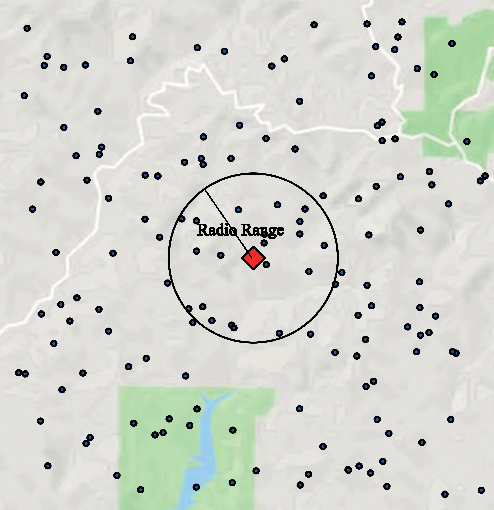
\includegraphics[width=1.7in]{./Figure/uniform.pdf}}
\vspace{0.03in}
\subfigure[Gaussian distribution]{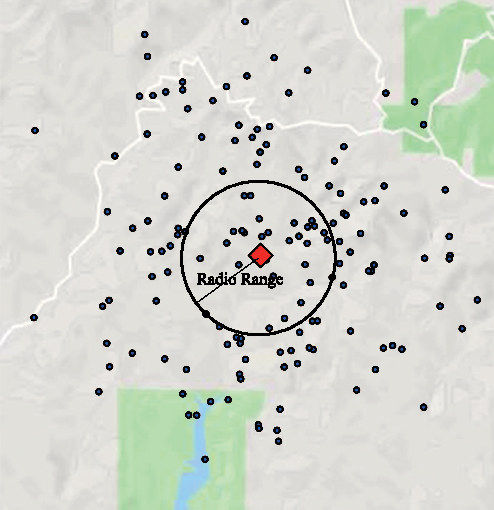
\includegraphics[width=1.7in]{./Figure/normal.pdf}}
\caption{WSN deployments following uniform and Gaussian distribution.}
\label{distribution}
%\vspace{-0.2in}
\end{figure}
\fi

Our insight idea is that, by estimating the expected number of neighbors of a node and aligning the time it turns on the radio with its neighbors, 
we can achieve both low-latency and energy-efficiency for neighbor discovery. 
We first take the distributions of nodes into consideration. As studied in \cite{wang2013gaussian}, nodes in a wireless sensor network are likely to follow a uniform or a Gaussian distribution for detecting aims. % (as shown in Fig. \ref{distribution}) 
According to the local density, a node can estimate the number of neighbors and calculate an optimal probability for action decisions. Then based on this, we propose Alano, %\footnote{Alano is the god of luck in Greek mythology.}
a nearly optimal probability based algorithm for a large-scale network. Finally, we involve the duty cycle mechanism, i.e. the fraction of time the radio is on (also called a sensor wakes up), and modify Alano by deterministic techniques to align the wake-up time between neighbors. Specifically, if all nodes have the same (symmetric) duty cycle, such as a batch of sensors have a default duty cycle setting, we propose a Relaxed Difference Set based algorithm (called RDS-Alano); if nodes have different (asymmetric) duty cycles, such as a sensor adjusts the duty cycle by the remaining energy, we propose a Traversing Pointer based algorithm (called TP-Alano).

Our simulations show the proposed Alano 
has lower latency, higher discovery rate, and better scalability %, and robustness, 
 compared to the state-of-the-art algorithms \cite{you2011aloha, sun2014hello, chen2015heterogeneous, bakht2012searchlight}
in a large-scale network.
Alano achieves $31.35\%$ to $ 85.25\%$ lower latency
and reaches nearly $100\%$ discovery rate within half time. 
When the number of nodes increases from 1000 to 9000, 
Alano shows 4.68 times to 6.51 times lower latency for neighbor discovery.
%In addition, Alano still keeps low latency robustly when 5\% to 30\% nodes are off duty. 


%\iffalse
%% Contribution summarize
The contributions of the paper are summarized as follows:
\begin{itemize}
\item[1)] We utilize nodes' distribution and propose Alano, a nearly optimal algorithm that achieves low-latency neighbor discovery for a large-scale network;
\item[2)] In an energy-restricted large-scale network, we propose RDS-Alano for symmetric nodes and TP-Alano for asymmetric nodes. Both algorithms achieve low latency for discovering neighbors and can prolong node's lifetime;
\item[3)] We conduct experiments for fundamental observation and extensive simulations for large-scale networks.  Alano achieves lower latency, higher discovery rate, and better scalability,
which promises a potential scalability of IoT in the future work.  %, and robustness compared with the state-of-the-art algorithms. 
\end{itemize}
%\fi

%% Remaining structure
The remainder of the paper is organized as follows. The coming section highlights some related works and puts forward vital problems that the existing algorithms remain. The system model and basic definitions are introduced in Section \ref{sectionmodel}. We present Alano and show the method to combine nodes' distribution in Section \ref{PCN}. We propose two modified algorithms (RDS-Alano, TP-Alano) for a energy-restricted large-scale network for both symmetric and asymmetric nodes in Section \ref{EEN}. The extensive simulation results are shown in Section \ref{Evaluation} and we conclude the paper in Section \ref{Conclusion}.




% Previous version

% Paper Logic Flow
% P1-P2 Background
% P3-P6 motivation
% P7-P11 contribution
% P12 structure

%% P1:
%% Define realistic network
%% General background
%% The situation&scenario our research applies to
%The growing interest in the Internet of Things (IoT) has resulted
%in a number of wide-area deployments of wireless networks \cite{qin2014software},
%such as wireless sensor networks \cite{yick2008wireless}, mobile campus networks
%\cite{hernandez2005comparative}, mobile gaming community \cite{cunningham2002optimizing}, etc.
%All these realistic networks possess multi-hop and large-scale characteristics obviously.

%
%% P2:
%% Why NB problem is related and important to the background in P1
%% Define what is neighbor and what is neighbor discovery problem
%% A brief introduction of the existing works and explain deterministic and probabilistic with one sentence each
%Neighbor discovery is a fundamental step of constructing a wireless network, based on
%which the network can implement further applications such as routing and broadcasting.
%The core target is for each node in the network to discover the nodes in its radio sensing range
%with one-hop communication, which are called neighbors.
%A number of existing methods \cite{dutta2008practical, kandhalu2010u,
%bakht2012searchlight, sun2014hello, chen2015heterogeneous,
%wang2015blinddate, qiu2016talk, mcglynn2001birthday,
%vasudevan2009neighbor, you2011aloha, song2014probabilistic} have been proposed
%to deal with this issue, some of which are based on deterministic techniques,
%those turn on the radio with deterministic sequences,
%while others are probabilistic approaches, those turn on the radio with different probabilities.
%
%
%% P3:
%% Crucial problem:  collision issue in a partially-connected network
%% What is a practical network model and define what is a partially-connected network
%Unfortunately, despite great efforts, neighbor discovery in a realistic network remains an open problem.
%The key issue lies in the collision condition in the large-scale networks.
%In a large-scale network, each node is only able to sense the
%nodes if their Euclidean distance is no more than a given threshold
%based on received signal strength \cite{moscibroda2006complexity, wang2013gaussian, wang2015connectivity}.
%We call this multi-hop wireless network connectivity as \emph{partially-connected}.
%
%
%% P4:
%% What issues will occur, if transferring the deterministic methods to the partially-connected network
%% On the one hand,
%On the one hand, the deterministic approaches only deal with the neighbor discovery problem for two nodes.
%When transferred to multiple nodes scenario, they can not solve the collision issue when more
%than one neighbors are transmitting simultaneously.
%
%
%% P5:
%% What issues will occur, if transferring the probabilistic methods to the partially-connected network
%% On the other hand,
%On the other hand, probabilistic approaches can deal with multiple nodes discovery well but only consider
%the network is fully-connected, the topology of which is a complete graph.
%Therefore in the large-scale network where the nodes are partially-connected,
%the probability adopted in these approaches can not be desirable
%and thus can not reduce the collision efficiently.
%To our best knowledge, no relevant researches
%have focused on the neighbor discovery problem in the large-scale networks
%where nodes are partially-connected.
%
%
%% P6:
%% Summarize our initiative insight
%Our initiative insight is to take the distribution of the nodes in the network
%into fully consideration, since in a wireless network the distribution of
%nodes' deployment directly plays a vital role in determining the intrusion
%detection capability of a communication device.
%
%% P7:
%% Our solution/contribution : we propose Alano algorithm based on the distribution of nodes for the partially-connected networks
%In this paper, we propose Alano\footnote{Alano is the god of luck in Greek mythology.},
%a nearly optimal probability based algorithm to discover neighbors in large-scale networks.
%As fully studied in \cite{wang2013gaussian} , the nodes in wireless sensor networks are likely to
%follow a uniform or a Gaussian distribution as showed in Fig. \ref{distribution},
%depending on the specific network applications, which is taken into consideration of the proposed Alano algorithm.
%
%
% \begin{figure}[!t]
%\centering
%\subfigure[uniform distribution]{\includegraphics[width=1.7in]{./Figure/uniform.eps}}
%\vspace{0.03in}
%\subfigure[Gaussian distribution]{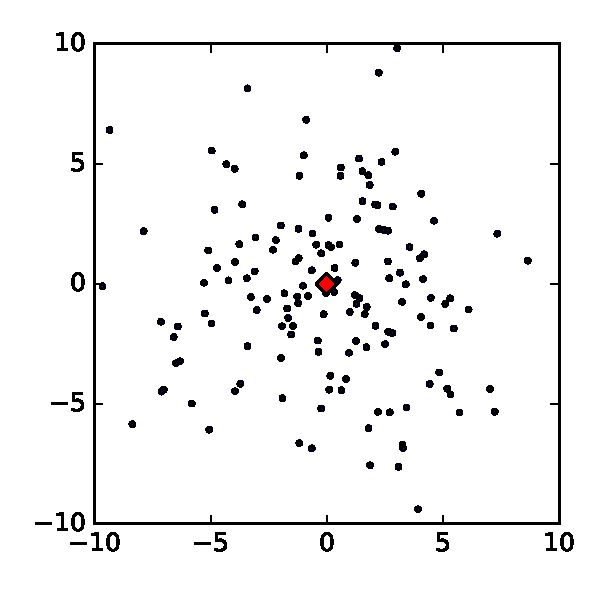
\includegraphics[width=1.7in]{./Figure/normal.eps}}
%\caption{WSN deployments following uniform and Gaussian distribution.}
%\label{distribution}
%%\vspace{-0.2in}
%\end{figure}
%
%
%% P8:
%% A special type of partially-connected networks: energy-efficient network
%In addition, among the large-scale networks, there is a special
%type named energy-efficient network \cite{jones2001survey}.
%Wireless sensor network is a typical energy-efficient network that all the sensor nodes have to maintain
%strict power budgets to attain years of lifetime\cite{dunkels2011contikimac}.
%Duty cycle mechanism, the fraction of time the radio is turned on, is
%utilized to raise the power-awareness of the nodes in the network.
%Correspondingly, the neighbor discovery process
%needs adjustments to deal with the dilemma between
%a balance of energy-efficiency and low-latency.
%
%
%% P9:
%% For energy-efficient networks, we propose RDS-Alano in global duty cycle scenario
%% and TP-Alano in the local duty cycle scenario.
%For energy-efficient networks, we design deterministic methods
%to align the wake-up time slots between the neighbors to achieve lower latency bound.
%Specifically, We propose RDS-Alano algorithm for the symmetric energy-efficient networks, where
%all the nodes share a identical duty cycle $\theta$ and TP-Alano for the
%asymmetric energy-efficient networks where each node possesses a respective duty cycle $\theta_i$.
%
%
%% P10:
%% Simulation results support our high performance
%Our simulation shows the proposed Alano algorithms
%hold significant strengths compared to the state-of-the-art methods,
%based on the evaluation of speed, quality, scalability and robustness.
%Alano achieves 31.35\% to 32.32 times lower latency
%and has higher discovery rate during the whole process of neighbor discovery,
%no matter in symmetric or asymmetric scenario and in uniform or Gaussian distribution.
%When the number of nodes increases and the network becomes denser,
%Alano still keeps its high performance.
%
%
%% P11:
%% Contribution summarize
%The main contributions of this paper are summarized as follows:
%\begin{itemize}
%\item[1)] We consider the distribution of nodes and propose Alano,
%a low-latency algorithm to achieve neighbor discovery process in a large-scale network.
%\item[2)] We propose a Relaxed Difference Set based Alano algorithm (RDS-Alano)
%to achieve low-latency neighbor discovery process in the symmetric energy-efficient networks.
%\item[3)] We propose a Traversing Pointer based Alano algorithm (TP-Alano) to
%achieve low-latency neighbor discovery process in the asymmetric energy-efficient networks.
%\end{itemize}
%
%
%% P12:
%% Remaining structure
%The remainder of the paper is organized as follows.
%The next section highlights some related work and
%puts forward some serious problems.
%Some notion definitions and the system model are given in Section \ref{sectionmodel}.
%We analyse the node's expected number of neighbors and
%propose Alano algorithm in \ref{PCN} as a foundation.
%Section \ref{EEN} describes the RDS-Alano algorithm for
%symmetric scenario and TP-Alano algorithm for asymmetric scenario
%respectively in energy-efficient networks.
%We have conducted extensive simulations, and the results are shown in Section
%\ref{Evaluation}. Finally, we conclude the paper in Section
%\ref{Conclusion}.

